\documentclass[journal]{new-aiaa}
% \documentclass[conf]{new-aiaa} %for conference papers
\usepackage[utf8]{inputenc}

\usepackage{graphicx}
\usepackage{amsmath}
\usepackage[version=4]{mhchem}
\usepackage{siunitx}
\usepackage{longtable,tabularx}
\setlength\LTleft{0pt}

% \usepackage{amsmath}          % for formula writing (i.e. 'split', etc)
\usepackage{rotate}           %rotate/mirror images
\usepackage{cancel}           %draw lines through math to show "goes to zero"
\usepackage{xfrac}            %allows slated and side fractions
\usepackage{subcaption}       %allows captioning individual subfigures
\usepackage[mode=buildnew]{standalone}% requires -shell-escape
  % compile with `pdflatex -shell-escape main` or `xelatex  -shell-escape main`

\usepackage{float} %Force figures to exact location in doc (use '[H]' option)

\usepackage{tikz}             %for creating vector graphics diagrams
\usetikzlibrary{backgrounds}  %put backgrounds behind tikz figures
\usetikzlibrary{calc}         %perform calculations within $$
\usetikzlibrary{positioning}  %position tikz elements using "right of, etc"
\usetikzlibrary{angles}       %label angles between lines with arcs
\usetikzlibrary{quotes}       %Put angle label in quotes
\usetikzlibrary{patterns}     %Patterns to fill shapes with




\title{Review of Analysis and Modeling Techniques for Incompressible, Turbulent Bluff-Body Wakes}

\author{Logan D. Halstrom\footnote{Graduate Student, Mechanical And Aerospace Engineering Department, One Shields Avenue} and Federico Zabaleta\footnote{Graduate Student, Civil and Environmental Engineering Department, One Shields Avenue}}
\affil{University of California, Davis, California, 95616}



%%%%%%%%%%%%%%%%%%%%%%%%%%%%%%%%%%%%%%%%%%%%%%%%%%%%%%%%%%%%%%%%%%%%%%%%
\begin{document}

\maketitle

%%%%%%%%%%%%%%%%%%%%%%%%%%%%%%%%%%%%%%%%%%%%%%%%%%%%%%%%%%%%%%%%%%%%%%%%
\begin{abstract} %%%%%%%%%%%%%%%%%%%%%%%%%%%%%%%%%%%%%%%%%%%%%%%%%%%%%%%
%%%%%%%%%%%%%%%%%%%%%%%%%%%%%%%%%%%%%%%%%%%%%%%%%%%%%%%%%%%%%%%%%%%%%%%%

\textcolor{red}{abstract here}
\textcolor{red}{\emph{LH\&FZ}}

\end{abstract}



%%%%%%%%%%%%%%%%%%%%%%%%%%%%%%%%%%%%%%%%%%%%%%%%%%%%%%%%%%%%%%%%%%%%%%%%
\section*{Nomenclature} %%%%%%%%%%%%%%%%%%%%%%%%%%%%%%%%%%%%%%%%%%%%%%%%
%%%%%%%%%%%%%%%%%%%%%%%%%%%%%%%%%%%%%%%%%%%%%%%%%%%%%%%%%%%%%%%%%%%%%%%%

\textcolor{red}{\emph{LH\&FZ}}

{\renewcommand\arraystretch{1.0}
\noindent\begin{longtable*}{@{}l @{\quad=\quad} l@{}}
$\rho$ & density, $kg/m^3$\\
\multicolumn{2}{@{}l}{Subscripts}\\
$()_{\infty}$ & freestream quantity\\
\multicolumn{2}{@{}l}{Acronyms}\\
CFD & Computational Fluid Dynamics\\
\end{longtable*}}



%%%%%%%%%%%%%%%%%%%%%%%%%%%%%%%%%%%%%%%%%%%%%%%%%%%%%%%%%%%%%%%%%%%%%%%%
\section{Introduction} \label{sec:intro}
%%%%%%%%%%%%%%%%%%%%%%%%%%%%%%%%%%%%%%%%%%%%%%%%%%%%%%%%%%%%%%%%%%%%%%%%




\lettrine{I}{ntro} sentence to paper should have this fancy capitalization.

\begin{itemize}
    \item Driving Physical Phenomena \textcolor{red}{\emph{FZ}}

    \begin{itemize}
        \item differences from potential flow
        \item blunt/bluff body definition, differences from streamlined body flow
        \item massively separated flow
        \item base pressure
        \item wake
    \end{itemize}
    \item Real World Applications \textcolor{red}{\emph{LH}}
    \begin{itemize}
        \item parachute
        \item reentry capsule
        \item vehicles
        \item buildings
        \item show similarity between cylinder/sphere wake and more complex bluff body
    \end{itemize}
\end{itemize}





%%%%%%%%%%%%%%%%%%%%%%%%%%%%%%%%%%%%%%%%%%%%%%%%%%%%%%%%%%%%%%%%%%%%%%%%
\section{Experimental Methods And Results} \label{sec:experimentalmethods}
%%%%%%%%%%%%%%%%%%%%%%%%%%%%%%%%%%%%%%%%%%%%%%%%%%%%%%%%%%%%%%%%%%%%%%%%

\textcolor{red}{\emph{FZ}}

\begin{itemize}
    \item Historical Study
    \item Experimental techniques
    \begin{itemize}
        \item ballistic range?
    \end{itemize}
    \item Applications
    \begin{itemize}
        \item Simple cases: cylinder/sphere
        \begin{itemize}
            \item Drag vs Re?
            \item Wake velocity profiles?
            \item Wake structure?
        \end{itemize}
        \item Sharp vs bluff: sphere vs cube
        \item Complex cases: capsule/building
    \end{itemize}
\end{itemize}








%%%%%%%%%%%%%%%%%%%%%%%%%%%%%%%%%%%%%%%%%%%%%%%%%%%%%%%%%%%%%%%%%%%%%%%%
\section{Computational Methods and Results} \label{sec:computationalmethods}
%%%%%%%%%%%%%%%%%%%%%%%%%%%%%%%%%%%%%%%%%%%%%%%%%%%%%%%%%%%%%%%%%%%%%%%%

\textcolor{red}{\emph{LH}}

\begin{itemize}
    \item Historical Study
    \item Computational techniques
    \item Applications
    \begin{itemize}
        \item Simple cases: cylinder/sphere
        \item Sharp vs bluff: sphere vs cube
        \item Complex cases: capsule/building
    \end{itemize}
\end{itemize}

%%%%%%%%%%%%%%%%%%%%%%%%%%%%%%%%%%%%%%%%%%%%%%%%%%%%%%%%%%%%%%%%%%%%%%%%
\subsection{Turbulence Modeling Aspects} \label{subsec:turbulencemodeling}

\textcolor{red}{\emph{LH}}

\begin{itemize}
    \item Compare turbulence model performance for sphere/cylinder
    \begin{itemize}
        \item SA
        \item SST
        \item SAS
        \item URANS
        \item LES
        \item DES
        \item DNS?
    \end{itemize}
\end{itemize}


LIST ALL FIGURES HEAR, REORDER AND DESCRIBE LATER

%%% CURVE BACKSTEP VELOCITY PROFILE LES VS RANS
    % SOURCE: ?
%%\vspace{-2em}
% \begin{figure}[htb]
\begin{figure}[H]
\begin{center}
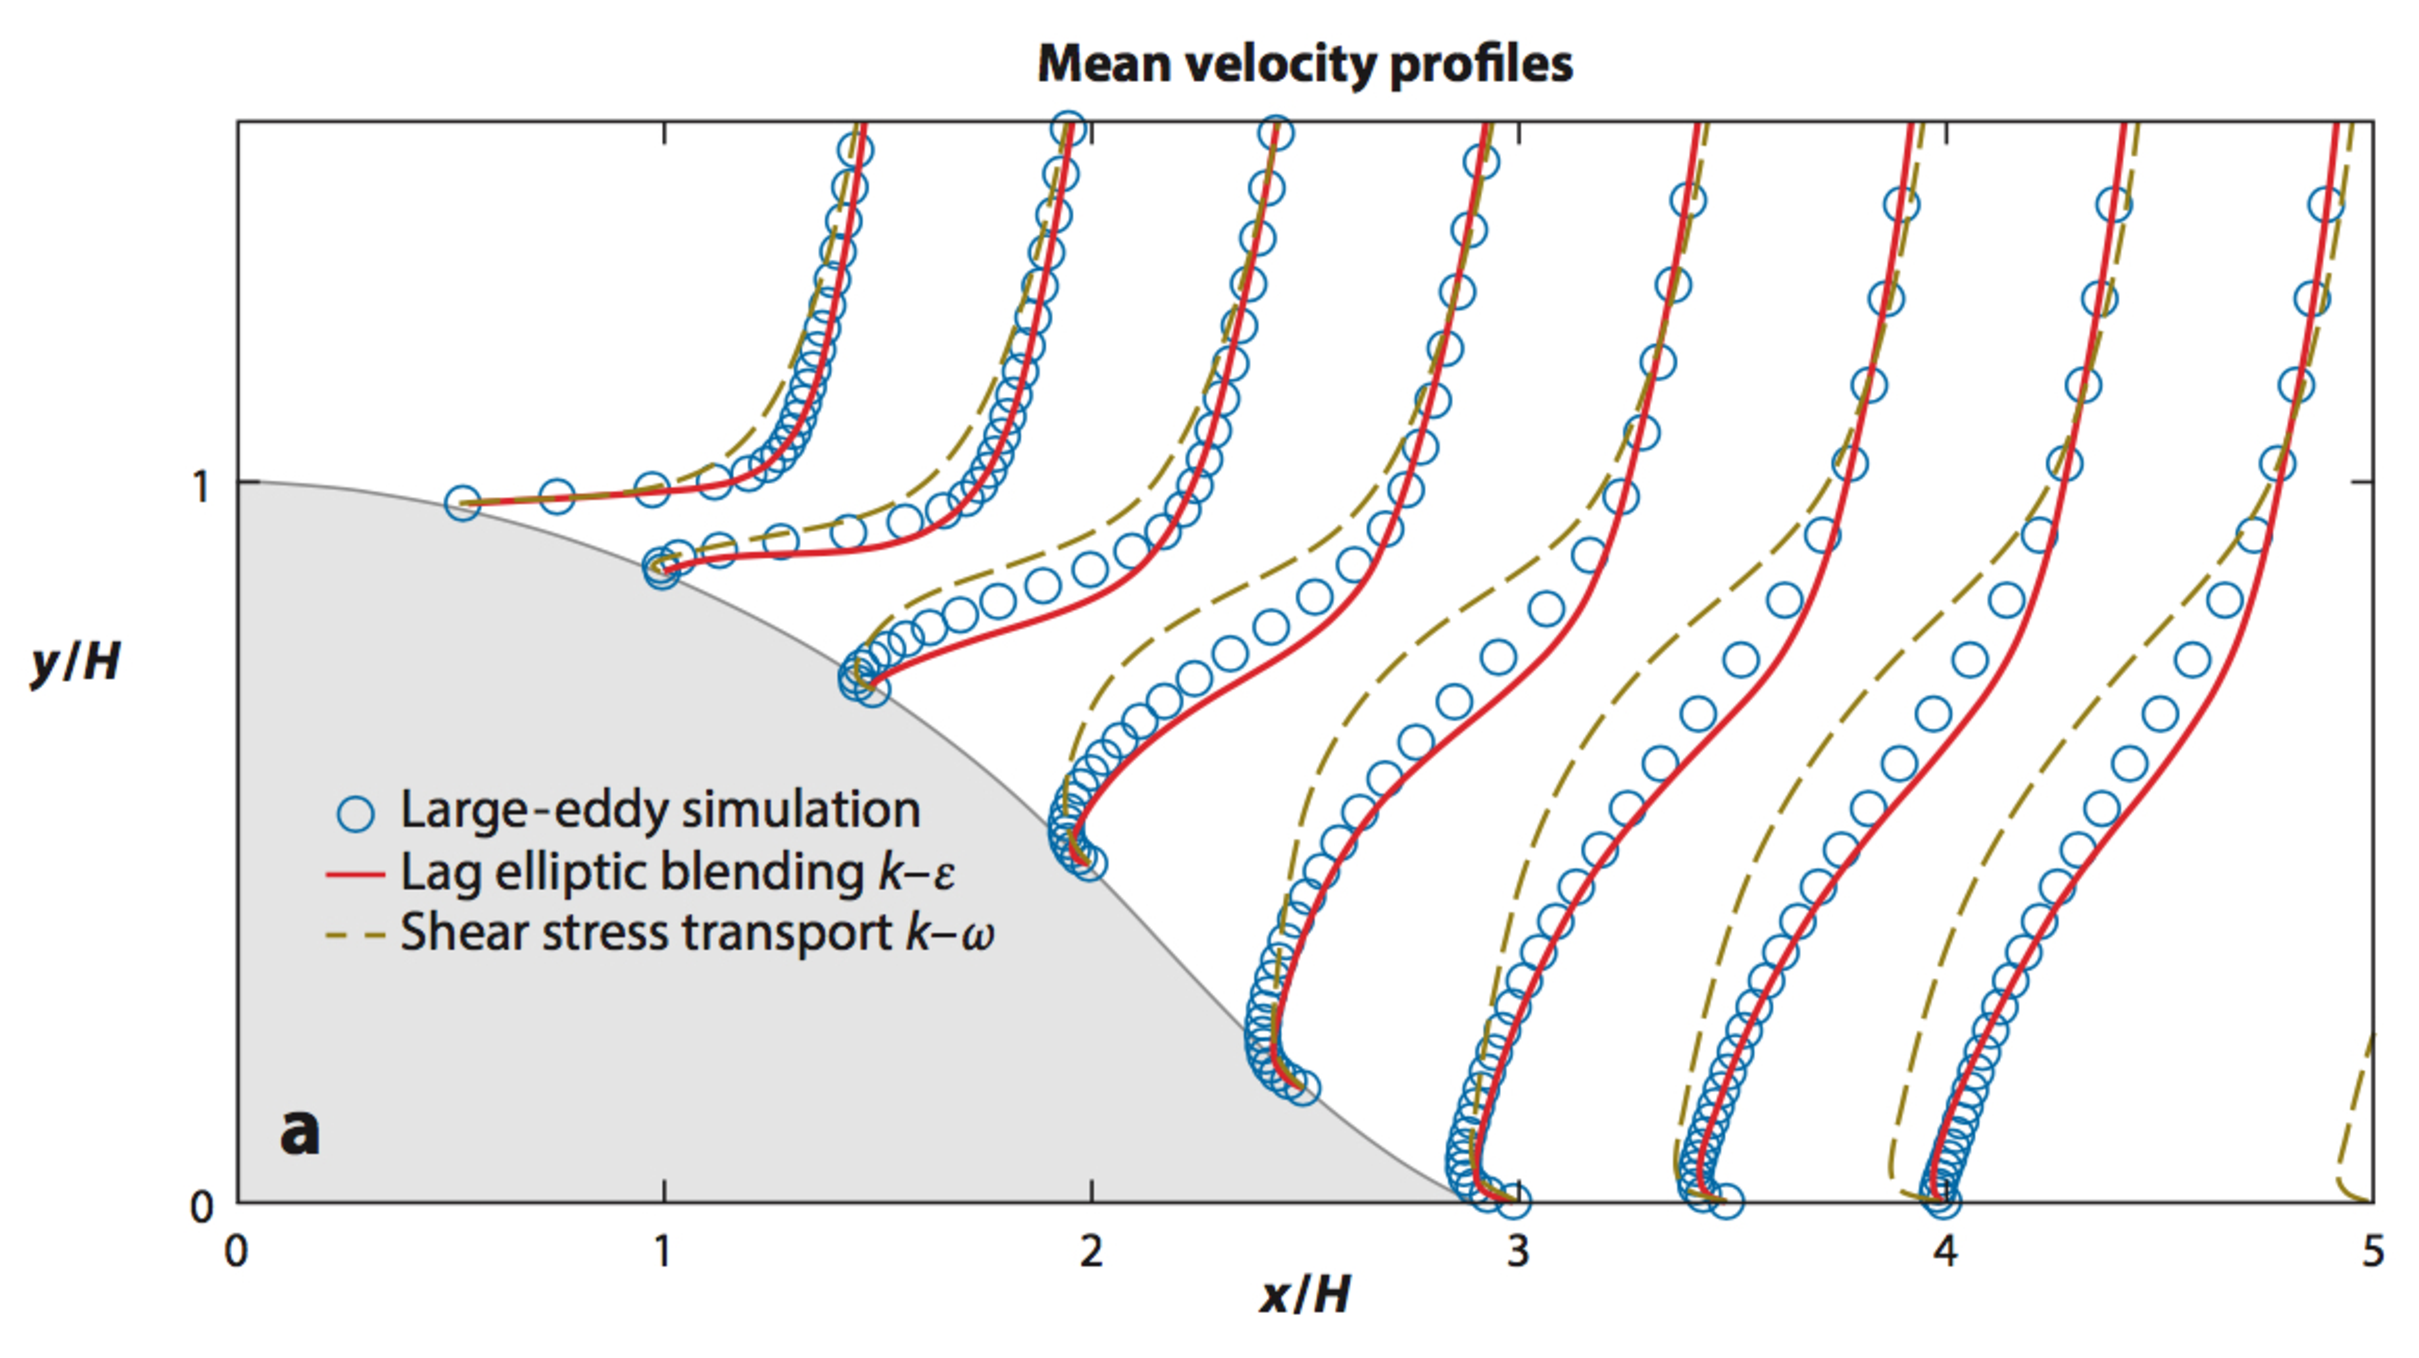
\includegraphics[width=0.5\textwidth]{Images/logan/durbin2018some_BackstepLESvsRANS.pdf}
\caption{curve backstep velocity profile les vs rans \cite{durbin2018some}}
\label{fig:backsteplesrans}
\end{center}
\end{figure}
%%\vspace{-2em}










%%%%%%%%%%%%%%%%%%%%%%%%%%%%%%%%%%%%%%%%%%%%%%%%%%%%%%%%%%%%%%%%%%%%%%%%
\section{Current State of Bluff-Body Turbulence Analysis} \label{sec:currentstate}
%%%%%%%%%%%%%%%%%%%%%%%%%%%%%%%%%%%%%%%%%%%%%%%%%%%%%%%%%%%%%%%%%%%%%%%%

\begin{itemize}
    \item Current State of Knowledge
    \item Remaining Challenges
\end{itemize}


%%%%%%%%%%%%%%%%%%%%%%%%%%%%%%%%%%%%%%%%%%%%%%%%%%%%%%%%%%%%%%%%%%%%%%%%
\subsection{Experimental Methods} \label{subsec:currentstateexperimental}

\textcolor{red}{\emph{FZ}}


%%%%%%%%%%%%%%%%%%%%%%%%%%%%%%%%%%%%%%%%%%%%%%%%%%%%%%%%%%%%%%%%%%%%%%%%
\subsection{Computational Methods} \label{subsec:currentstatecomputational}



\textcolor{red}{\emph{LH}}














%%%%%%%%%%%%%%%%%%%%%%%%%%%%%%%%%%%%%%%%%%%%%%%%%%%%%%%%%%%%%%%%%%%%%%%%
\section{Conclusions}
%%%%%%%%%%%%%%%%%%%%%%%%%%%%%%%%%%%%%%%%%%%%%%%%%%%%%%%%%%%%%%%%%%%%%%%%

\textcolor{red}{\emph{LH\&FZ}}



%%%%%%%%%%%%%%%%%%%%%%%%%%%%%%%%%%%%%%%%%%%%%%%%%%%%%%%%%%%%%%%%%%%%%%%%
\section*{Acknowledgments} %%%%%%%%%%%%%%%%%%%%%%%%%%%%%%%%%%%%%%%%%%%%%
%%%%%%%%%%%%%%%%%%%%%%%%%%%%%%%%%%%%%%%%%%%%%%%%%%%%%%%%%%%%%%%%%%%%%%%%

\textcolor{red}{\emph{LH\&FZ}}

%%%%%%%%%%%%%%%%%%%%%%%%%%%%%%%%%%%%%%%%%%%%%%%%%%%%%%%%%%%%%%%%%%%%%%%%
%%% BIBLIOGRAPHY %%%%%%%%%%%%%%%%%%%%%%%%%%%%%%%%%%%%%%%%%%%%%%%%%%%%%%%
%%%%%%%%%%%%%%%%%%%%%%%%%%%%%%%%%%%%%%%%%%%%%%%%%%%%%%%%%%%%%%%%%%%%%%%%

%SAMPLE CITATIONS TO SEE CITATION FORMATTING
\textcolor{red}{Example citations}

\cite{nakamura1993bluffbody}

%bibliography from .bib file, filename goes in {}
%NOTE: References must be cited with "\cite" command to appear in bibliography
%Types of Refs: article, book, conference=inproceedings, manual, mastersthesis, phdthesis, techreport, unpublished, misc (see "new-aiaa.bst")
%when you first initialize .bib file, might need to have plain text in front of \cite command to get sublime text to recognize bibliography file
\bibliography{BluffBodyTurb}

\end{document}
